\documentclass[11pt,twocolumn,varwidth=true,a4paper,fleqn]{sigchi}
\usepackage{fullpage}
\usepackage{url}
\usepackage[margin=1.1in]{geometry}
\usepackage{graphicx}
\usepackage{csvsimple}
\usepackage{varwidth}
\usepackage{array}
\usepackage{float}
\usepackage{amsmath}
\usepackage{pgfplotstable}
\usepackage{amsmath }
\usepackage[T1]{fontenc}
\usepackage[compact]{titlesec}
\usepackage{authblk}

\author[1]{Bernstein Ran}
\author[2]{Shafir Tal}
\author[3]{Tsachor Rachelle}
\author[4]{Studd Karen}
\author[1]{Schuster Assaf}
\affil[1]{Department of Computer Science, Technion I.I.T, Haifa, Israel}
\affil[2]{The Graduate School of Creative Arts Therapies, University of Haifa}
\affil[3]{School of Theatre \& Music, The University of Illinois at Chicago}
\affil[4]{School of Dance, George Mason University}

\begin{document}
\nocite{*}

\title{Multitask Learning for LMA}
\date{}
\maketitle

\begin{abstract}
\textbf{Laban Movement Analysis (LMA) is a method for describing, interpreting
and documenting all varieties of human movement.
Analyzing movements using LMA is advantageous over kinematic description,
as it captures their qualitative aspects in addition to the quantitative.
Thus, in recent years, LMA is increasingly becoming the preferred method for movement analysis.
In this study we examine a multitask Learning approach for recognizing Laban qualities from a
markerless Motion Capture (MOCAP) camera --- Microsoft's Kinect. This approach
has obtained an improvement  in recall and precision rate of about 60\%  --- 4\%
more than single learning that appears in earlier work. In addition, an
evaluation on a never seen CMAs and a non CMAs were made.}
\end{abstract}

\section{Introduction}

LMA is a formal language for motion description first developed by Rudolf Laban \cite{Laban} and colleagues in the middle of the 20th century.
LMA describes both conscious and unconscious human movement, based on Laban's categories of \textit{Body}, \textit{Effort}, \textit{Shape}, and \textit{Space}.
LMA has been used in the fields of dance, acting, athletics, physical therapy, and psychology and behavioral science.
LMA helps actors create momentary moods and portray personality traits through
movement. For example, LMA work investigates the \textit{Effort} properties
\textit{Flow}, \textit{Space}, \textit{Time} and \textit{Weight} of all movement and helps actors
think specifically about why their character might move in a jerky, fast, light and direct manner
versus a heavy, slow, indirect and uninterrupted manner.
The entire LMA hierarchy is shown in figure \ref{labanTree}.
\begin{figure*}[ht]
\centering
\caption{Main axes of LMA. Taken from  }\cite{labanTree}
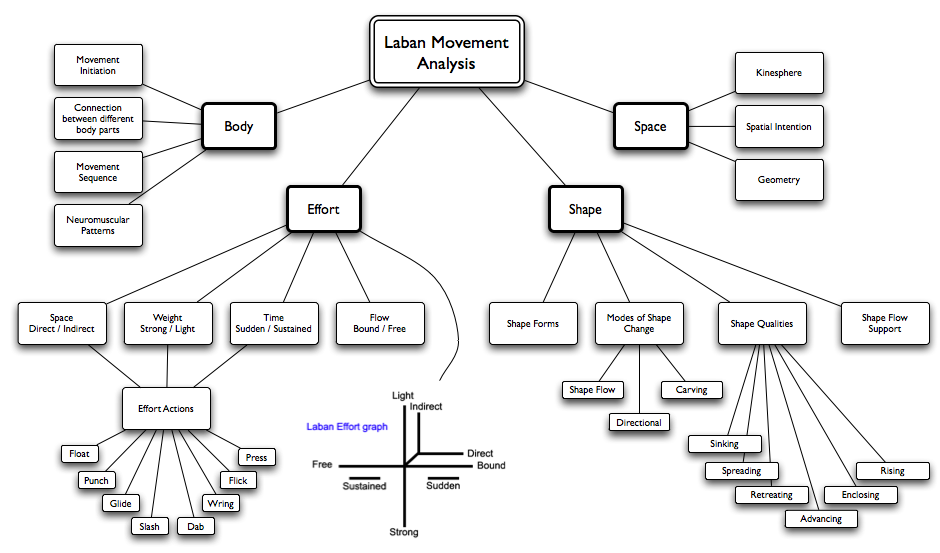
\includegraphics[width=\textwidth]{laban.png}
\label{labanTree}
\end{figure*}

\mbox{}
\par
There are numerous applications for computerized identification of the
qualities that characterize each possible human movement. Examples include the generation and control of specific expressive movements of avatars, virtual characters, or robots in mixed reality scenarios
\cite{Masuda}; detection of personality traits during a job interview
\cite{levy2003use}; early detection, severity assessment or revealing of genetic tendency (phenotype) towards various illnesses such as Alzheimer's,
autism, Parkinson's disease \cite{camurri2003application}, or schizophrenia,
based on analysis of the person's motor behavior. Automated emotion recognition from movement is another
important application, which may have a variety of uses such as online feedback
to presenters to help them convey through their body language the emotional message they want to communicate
(e.g., politicians and public speakers or actors in training) \cite{nguyen2012online}; or recognition
of people's emotions during interactive games such as those played using the Xbox \cite{Zacharatos}.
\mbox{}\\
\par
Several attempts were made to recognize Laban qualities. The first was Chi
et al. \cite{chi2000emote}, who quantified \textit{Effort} and \textit{Shape} for animation.
Most of the other attempts were for emotion recognition in the context of Human Robot Interaction (HRI).
Masuda et al. generated emotional body motion for a human form robot \cite{Masuda}.
Rett et al. proposed a human motion recognition system using a Bayesian reasoning framework \cite{Rett}.
The second line of works focused on LMA (not on emotions), but not using Kinect.
Lourens et al. \cite{lourens2010communicating} used video data and Samadani et al.
\cite{samadani2013laban} used a high quality MOCAP camera, but both of them
analyzed only hand gestures. A third line of works used Kinect as the main
sensor for skeletal information. Gabel et al. \cite{gabel2012full} used Kinect for gait analysis. The work of
Zacharatos et al. \cite{Zacharatos} was inspired by LMA for emotion recognition using Kinect. 
His feature extraction method was influenced by LMA principles, but he did not attempt to 
recognize the qualities themselves. Kim et al. \cite{kim} did attempt to do so but not on 
a real dataset and their work did not include a performance evaluation. Our work
continues Bernstein's et al. work \cite{ran}, but with multitask instead of
single-task learning and with analysis on people that are not CMA.
\mbox{}\\
\par
Our goal is to create a method for automated identification of Laban qualities that
characterize any movement sequence, using Kinect.
Our problem presents three challenges. The first is
quantifying subtle qualities for which a well-defined quantification has not yet been found.
The second challenge is handling noisy sensory data with an in-home setup, and the
third is keeping our method as general as possible --- We are developing a system capable of
handling different scenarios (dancing and acting, for example), and different postures
(sitting and standing, for example), by different people of different backgrounds (if any)
in movement. For reducing our data collection and analysis effort, we focused our work on 18 Laban qualities
(as listed in table \ref{mixedSummary}) that have been found predictive for emotional state
\cite{ShafirPrivate}.

\section{Method}
\subsection{Kinect Sensor Data}
Figure \ref{skeleton} shows the skeleton provided by Kinect's SDK.
\begin{figure}[h]
\centering
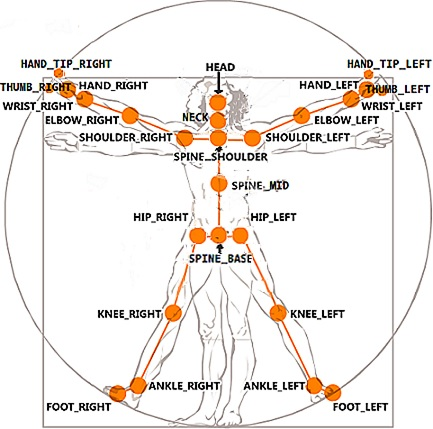
\includegraphics[width=60mm]{skeleton.jpg}
\caption{Skeleton positions relative to the human body}
\label{skeleton}
\end{figure}
Once the skeleton is detected, the 3D coordinates of all the joints of the
user's body --- with the exception of joints that are not visible (e.g., a user's
hand is behind his or her back) --- are provided.
As seen in Figure \ref{Coordinate}, the coordinates are in a ``real-world''
coordinate system, whose origin [0,0,0] is in the sensor and whose x-, y-, and
z-axis are as depicted below.
\begin{figure}[h]
\centering
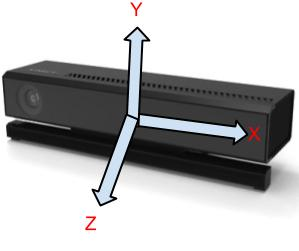
\includegraphics[width=60mm]{KinectV2CoordinateSystem.jpg}
\caption{Kinect Coordinate System}
\label{Coordinate}
\end{figure}

\subsection{Clip Collection}
Two main datasets were collected:
\begin{itemize}
  \item
  CMA dataset - includes 6 CMAs performing in about
  80 clips each (a total of 550 clips). Every clip is about 3 seconds long, 
  and the CMAs executed combinations of the 18 qualities.
  To achieve uniform distribution of the Laban qualities over the dataset, in every
  clip the CMA was asked to perform actions that include several specific qualities,
  and nothing but them.
  
  \begin{figure}[h]
\centering
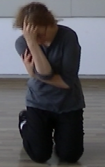
\includegraphics[width=30mm]{Rachelle.png}
\caption{CMA during a clip}
\label{Rachelle}
\end{figure}

\item
Non-CMA dataset - includes 5 subjects that are not CMAs, performing 30 clips each. 
Every clip is also about 3 seconds long, and the subject was asked to perform one out 
of several every day tasks.
\end{itemize}
\subsection{Clip Labeling}
To achieve a ground truth labeling for the two datasets, every clip was tagged by
a committee of 2 CMAs who determined which Laban qualities appear in the
clip. The use of a committee decision instead of the subjective opinion of one
CMA decreases the labeling noise and the decision is considered as ground truth.
\subsection{Feature Extraction}
The feature extraction is adopted from an earlier work \cite{ran}.
Due to the unequal length of clips, all the extracted features are in whole clip 
granularity. We extracted two groups of features, the first is a relatively
small, and contains about 100 features that each one of them is designed for a
specific quality. The second group contains about 6000
features, and exploits the rich data that is provided by Kinect, by extracting from every joint in the skeleton, the
angular velocity, acceleration, and jerk. For every joint/metric pair, the mean,
variance, skew, and kurtosis were extracted. 

\subsection{Multitask Learning}
The multitask learning framework \cite{caruana1997multitask},  tries to learn multiple tasks simultaneously even
when they are different. The goal of MTL is to improve the performance of learning algorithms by learning
classifiers for multiple tasks jointly. This works particularly well if these tasks have some commonality and
are generally slightly under sampled.
For the multitask setting we used Multitask Elastic Net (MEN) regularization, which is
the multitask regularization method of Zou et al. \cite{Zou}, where the
optimization objective is:
\\
\begin{equation}\label{eq:MEN}
\|Y - XW\|^2_F+\lambda_1\cdot\|W\|_{2,1}+\lambda_2\cdot\|W\|^2_F,
\end{equation}

$\lambda_1$, and $\lambda_2$ are hyper-parameters, where,
\\
\begin{equation*}
\|W\|_{2,1} = \sum_i \sqrt{\sum_j w_{ij}^2},
\end{equation*}
i.e., the sum of norm of each row (also known as mixed norm), and
\begin{equation*}
\|W\|^2_F = \sum_i{\sum_j w_{ij}^2},
\end{equation*}
i.e., the Frobenius norm.
Feature selection was carried out by averaging the statistical significance of
each feature with respect to all of the tasks (this is in contrast to the single
task learning flow, where every task had its own feature selection). As seen in
Table \ref{MultitaskVsSeparated}, the multitask setting improved the F score by
7\%, indicating that the tasks are correlated and more might be learned
from the small dataset when using this setting.

\section{Experimental Setups and Results}
\subsection{Multitask vs Single Task Learning}
We found that multitask learning for all the 18 qualities together exhibited superior
performance to learning a classifier for each problem separately.
\begin{table}[ht]
\centering
\begin{tabular}{|p{1.8cm}|p{1.8cm}|p{1.8cm}|}
\hline
Metric&Single task&Multitask\\\hline
Precision&0.46&\textbf{0.59}\\\hline
Recall&\textbf{0.71}&0.65\\\hline
F1&0.56&\textbf{0.6}\\\hline
\end{tabular}
\caption{Multitask vs Single task learning performance evaluation on a CMA mixture
dataset.}
\label{MultitaskVsSeparated}
\end{table}

\subsection{Performance of Every Quality}
The performance over every quality as classified by the MEN in Table
\ref{mixedSummary}. During the MEN optimization ~\eqref{eq:MEN}, the mixed norm
term $\|W\|_{2,1}$  promotes sparsity in the weights matrix $W$ such that for
every row in the matrix, if one coordinate is equal to zero, then every coordinate
in the row will be equal to zero.
\\The generalization ability of the model was enhanced by the fact that the
decision which features to select is influenced by all the qualities, (feature $f_i$ is
selected in the MEN if the row $r_i$ in $W$ is not all zeros). The most
significant improvement were in the qualities that performed worse in the
single task learning setting (\textit{Strong} and \textit{Sudden} for example).
\begin{table}[!h]
\centering
\begin{tabular}{|p{3cm}|p{0.9cm}|p{0.9cm}|p{0.9cm}|}
\hline
Quality&Precis-ion&Recall&F1 score\\\hline
Jump&0.89&0.81&0.85\\\hline
Twist and Back&0.69&0.85&0.76\\\hline
Sink&0.62&0.79&0.69\\\hline
Rhythmicity&0.59&0.72&0.65\\\hline
Spread&0.55&0.76&0.64\\\hline
Head drop&0.60&0.66&0.63\\\hline
Rotation&0.66&0.60&0.63\\\hline
Free and Light&0.45&0.94&0.61\\\hline
Up and Rise&0.67&0.54&0.60\\\hline
Condense and Enclose&0.44&0.84&0.58\\\hline
Arms To Upper Body&0.67&0.54&0.60\\\hline
Advance&1.00&0.38&0.55\\\hline
Retreat&0.50&0.59&0.54\\\hline
Passive&0.40&0.85&0.54\\\hline
Bind&0.44&0.61&0.51\\\hline
Direct&0.56&0.49&0.52\\\hline
Sudden&0.61&0.41&0.49\\\hline
Strong&0.29&0.42&0.34\\\hline
\textbf{Average}&\textbf{0.59}&\textbf{0.65}&\textbf{0.60}\\\hline
\textbf{SD}&\textbf{0.17}&\textbf{0.17}&\textbf{0.11}\\\hline
\end{tabular}
\caption{Recall, precision and F1 score of each Laban quality on a CMA
mixture dataset. The learning was done in a multitask setting. The number of
features that weren't nullified by the mixed norm regularization is
282 (same features for all of the tasks). The F1 average and standard
deviation over the qualities is shown in the last row of the table.}
\label{mixedSummary}
\end{table}

\subsection{Evaluation on an Unseen CMA}
In this experiment the test set was taken from a CMA who did not appear in the train set.
As shown in Figure \ref{domainAdaptationBaseLine}, performance degrades on the unseen CMA from 0.6 to 0.57.
We blame the degradation on the large variability between clips from one CMA to another. 
Every CMA performed different gestures, in different postures (some sitting and some standing) 
and in different contexts (some were dancing while some were acting).

\begin{figure}[!h]
\centering
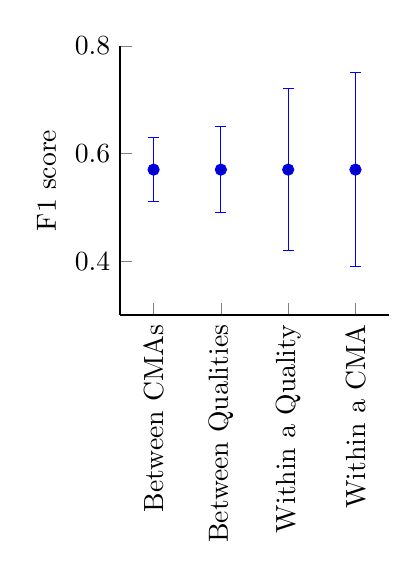
\begin{tikzpicture},
\centering
\begin{axis}[
height=5cm,
width=5cm,
ylabel={F1 score},
ymax=0.8,
ymin=0.3,
xmin=0.5,
xmax=4.5,
axis y line*=left,
axis x line*=bottom,
xticklabels={Between CMAs, Between Qualities, Within a Quality, Within a CMA},
xtick={1,2,3,4},
x tick label style={rotate=90,anchor=east}]
\addplot+[only marks][error bars/.cd,y dir=both, y explicit]
coordinates {
(1,0.57) +- (0.06,0.-0.06)
(2,0.57) +- (0.08,0.08)
(3,0.57) +- (0.15,-0.15)
(4,0.57) +- (0.18,-0.18)
};
\addplot[dashed] coordinates {(0,0) (10.5,0)};
\end{axis}
\end{tikzpicture}
\caption{Confidence intervals of F1 score in quality detection of an unseen CMA.
Every confidence interval is two standard deviations (STD) long.
In every trial one CMA was the test set, while the classifier was trained on the rest. The mean F1 score is 0.57. The measures from left to right are: STD between CMAs when every CMA's score is an average the scores of his or her qualities; STD between qualities when every quality's score is an average of all of the CMAs' scores for this quality; an average of qualities' STDs, where every STD is between CMAs within a quality; an average of CMAs' STDs, where every STD is between qualities within a CMA's dataset.}
\label{domainAdaptationBaseLine}
\end{figure}

\subsection{Validation on Ordinary People}
The final validation was conducted on ordinary people (non-CMAs). We
designed several daily actions (greeting friends or playing with a balloon, for
example) and the CMA committee tagged the clips. This dataset was small, with a
focus on the qualities that we found easier to recognize. The evaluation is shown in Figure \ref{nonCMAs}.

\begin{figure}[ht!]
\centering
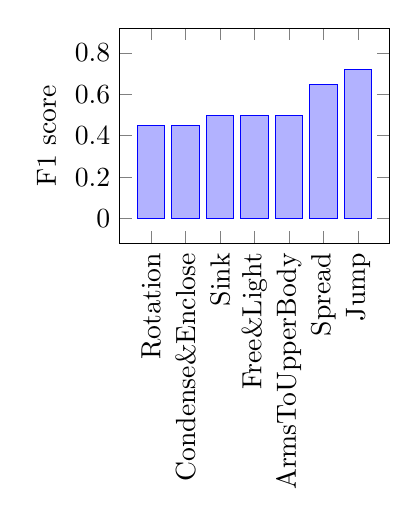
\begin{tikzpicture}
\begin{axis}[
ymin=0,
ymax=0.8,
width=5cm,
ybar stacked,
enlargelimits=0.15,
ylabel={F1 score},
symbolic x coords={Rotation,Condense\&Enclose,Sink,Free\&Light,ArmsToUpperBody,Spread,Jump},
xtick=data,
x tick label style={rotate=90,anchor=east},
]
\addplot+[ybar] plot coordinates  {(Rotation,0.45) (Condense\&Enclose,0.45) (Sink,0.5)
(Free\&Light,0.5) (ArmsToUpperBody,0.5) (Spread, 0.65) (Jump,0.72)};

\end{axis}
\end{tikzpicture}
\caption{Performance on ordinary people (non-CMAs) instructed to
perform several tasks.}
\label{nonCMAs}
\end{figure}

\section{Conclusion}
\\\\The improvement of the F1 score from a single task learning setting (0.56) to a multitask
setting (0.6) demonstrates the synergy of a shared model for several correlated tasks.
The mild degradation of the F1 score from a seen CMA (0.6) to an unseen (0.57) shows
a very good generalization ability of our linear classification model.
This ability derives from our focus on the MEN regularization terms, which resulted in our
model being not too rich, even sparse, and thus not over-fitted.
\bibliographystyle{unsrt}
\bibliography{bib}

\end{document}
